% Gemini theme
% https://github.com/anishathalye/gemini

\documentclass[final]{beamer}

% ====================
% Packages
% ====================

\usepackage[T1]{fontenc}
\usepackage{lmodern}
\usepackage[size=custom,width=91,height=122,scale=1.0]{beamerposter}
\usetheme{gemini}
\usecolortheme{heriotwatt}
\usepackage{graphicx}
\usepackage{booktabs}
\usepackage{tikz}
\usepackage{pgfplots}
\usepackage{multicol}

% ====================
% Lengths
% ====================

% If you have N columns, choose \sepwidth and \colwidth such that
% (N+1)*\sepwidth + N*\colwidth = \paperwidth
\newlength{\sepwidth}
\newlength{\colwidth}
\newlength{\doublecolwidth}
\setlength{\sepwidth}{0.025\paperwidth}
\setlength{\colwidth}{0.3\paperwidth}
% 2 columns + separator
\setlength{\doublecolwidth}{0.625\paperwidth}

\newcommand{\separatorcolumn}{\begin{column}{\sepwidth}\end{column}}

% ====================
% Title
% ====================

\title{Improving Robustness of Dialog Systems in a \\ Data-Efficient Way with Turn Dropout}

\author{Igor Shalyminov \and Sungjin Lee}

\institute{\begin{tabular}[h]{ccccccc}
      & & &Heriot-Watt University & & & Microsoft Research \\
      & & &Edinburgh, UK & & &  Redmond, USA \\
      & & &\texttt{is33@hw.ac.uk} & & & \texttt{sule@microsoft.com}
  \end{tabular}
}

% ====================
% Body
% ====================

\begin{document}

\begin{frame}[t]
\begin{columns}[t]

\separatorcolumn

\begin{column}{\colwidth}
\begin{alertblock}{The problem}
Neural network-based dialog models often lack robustness to anomalous, out-of-domain (OOD) user input which leads to unexpected dialog behavior and thus considerably limits such models' usage in mission-critical production environments. The problem is especially relevant in the setting of dialog system bootstrapping with limited training data and thus no access to OOD examples. In this paper, we explore the problem of robustness of such systems to anomalous input and the associated  trade-off in accuracies on seen and unseen data.
\end{alertblock}

\begin{block}{A dataset for studying dialog systems' robustness}

We created a corpus of dialogues to study OOD robustness in a controlled environment using \texttt{bAbI+ tools}, i.e. we augmented bAbI Dialog Task 6 (Dialog State Tracking Challenge 2) with user's utterances from several other domains:
\begin{itemize}
    \item Frames dataset~\textemdash{} travel booking (1198 utterances),
    \item Stanford Key-Value Retrieval Network Dataset~\textemdash{} calendar scheduling, weather information retrieval, city navigation (3030 utterances),
    \item Dialog State Tracking Challenge 1~\textemdash{} bus information (968 utterances).
\end{itemize}

Our OOD augmentations are as follows:
\begin{itemize}
  \item \textit{turn-level OOD}: user requests from a foreign domain~\textemdash{} the desired system behavior for such input is the fallback action,
  \item \textit{segment-level OOD}: interjections in the user in-domain requests~\textemdash{} treated as valid user input and is supposed to be handled by the system in a regular way.
\end{itemize}

With these two augmentation types, we modelled a specific dialog pattern of interest: one of more user's OOD turns followed by self-correction and return to IND input (see Table \ref{tab:augmentation_example}).

For segment-level OOD, we mined utterances with the explicit affirmation of a mistake from Twitter and Reddit conversations datasets (e.g. ``my mistake'', ``I'm so sorry'')~\textemdash{} 701 and 500 utterances respectively.
Our datasets, as well as the tools for OOD-augmentation of arbitrary datasets of interest are openly available.
\end{block}

\begin{alertblock}{Example dialog}

\begin{table}
  \centering
  \small
    \begin{tabular}{c|l|p{0.85\columnwidth}}
      1&\textit{sys:}&Hello, welcome to the Cambridge restaurant system. You can ask for restaurants by area, \\
      &&price range or food type. How may I help you?  \\
      2&\textit{usr:}&\textbf{I'd like to get away from Monday, August 15, 2016 to Wednesday, August 31, 2016.} \\
      &&\textbf{My budget is \$3200 and I would leave from Detroit.} \\
      3&\textit{sys:}&Sorry I didn't catch that. Could you please repeat? \\
      4&\textit{usr:}&\textbf{Will there be frost in Durham next week?}\\
      3&\textit{sys:}&Sorry I didn't catch that. Could you please repeat? \\
      4&\textit{usr:}&\textbf{\textit{So sorry man}} I want a moderately priced restaurant in the west part of town \\
      5&\textit{sys:}&$<$api call$>$
    \end{tabular}
    \caption{Augmented dialog example (OOD content in bold, segment-level in italics)}
    \label{tab:augmentation_example}
\end{table}
\end{alertblock}
\end{column}

\separatorcolumn

\begin{column}{\doublecolwidth}
\begin{block}{Model architecture}
\begin{figure}
\centering
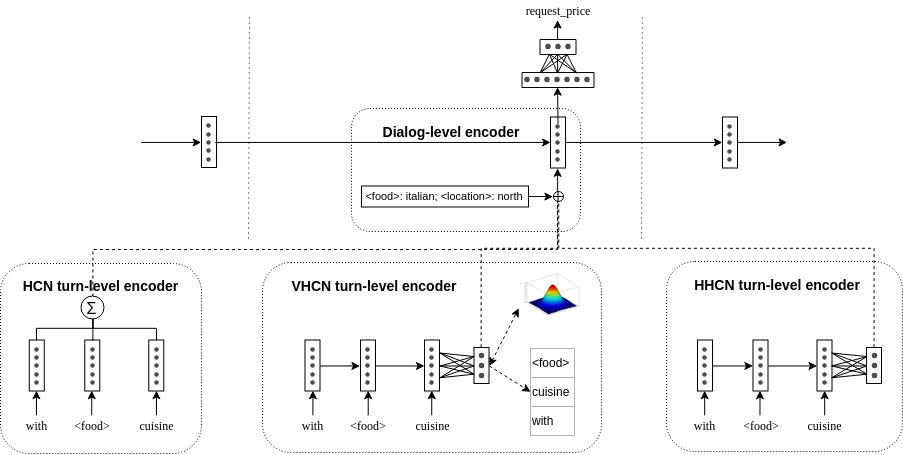
\includegraphics[scale=1.2]{img/hcn_all.png}
\caption{Hybrid Code Network-family models}
\label{fig:hcn_all}
\end{figure}
\end{block}

\begin{columns}[t,totalwidth=\doublecolwidth]

\begin{column}{\colwidth}
\begin{block}{Models}
We experiment with \textit{Hybrid Code Network} family of models. HCN is reported to be state-of-the-art for the original, IND-only bAbI Dialog Task 6 data~\textemdash{} in this paper, we explore its robustness to OOD input.

%HCN is a hierarchical dialog control model with a turn-level and a dialog-level encoders. The turn-level encoder produces a latent representation of a single dialog turn, and the dialog-level one augments it with additional dialog-level features (e.g. indicators of which slot values have been provided and whether the latest API call returned any results). Dialog-level encoder (RNN-based for all the models described) outputs a latent representation of the entire dialog which is then fed into the predictor MLP. Its output is the sequence of dialog actions (restricted by binary action masks provided by domain experts).

Our models share dialog-level encoder and dialog act predictor, and they only differ on the turn level and in the overall optimization objective (see Figure \ref{fig:hcn_all}).
\textit{The original \textbf{HCN}} encodes user's input turn $x$ consisting of $N$ tokens as follows:
\begin{equation} \label{eq:w2v}
HCN(x) = \frac{1}{N} \sum_i{w2v(x_i)}
\end{equation} where $w2v$ is the pre-trained Google News word2vec embeddings (frozen at the training time). HCN's optimization objective is categorical cross-entropy with respect to log-likelihood:
\begin{equation} \label{eq:l_hcn}
\mathcal{L}_{HCN} = \log p(a \mid x, c)
\end{equation} where $a$ is the dialog action and $c$ is dialog context.

\textit{\textbf{Hierarchical HCN (HHCN)}} uses an RNN (in our case an LSTM cell) for encoding each utterance:
\begin{equation} \label{eq:hhcn}
HHCN(x) = LSTM(x)
\end{equation}

The optimization objective is the same as of HCN.

\textit{\textbf{Variational HCN (VHCN)}}~\textemdash{} the model we are introducing here~\textemdash{} uses a Variational Autoencoder for generating turn-level latent code $z$:
\begin{equation}
VHCN(x) = \mu(LSTM(x)) + \sigma(LSTM(x)) * N(0, 1)
\end{equation}
 
Where $\mu$ and $\sigma$ are MLPs for predicting $z$'s posterior distribution parameters, and $N(0, 1)$ is a sample from its prior distribution, a standard Gaussian.
 
%In order to keep the secondary task less complex than the main one, we represent VAE's reconstruction targets as bags of words (BoW).
VHCN optimization objective is as follows:
\begin{equation} \label{eq:l_vhcn}
\begin{split}
 \mathcal{L}_{VHCN} & = \mathbb{E}_{q(z)}[log(p(a \mid z, c))] & + \mathbb{E}_{q(z)}[p(x_{BoW} \mid z)] & - KL(q(z\mid x) \mid\mid p(z))
 \end{split}
 \end{equation}

In this objective, bag-of-words representation of the input $x_{BoW}$ is used for the secondary task (input reconstruction, 2nd term) in order to lower the task's complexity. It also helps keep the variational properties of the model (i.e. non-zero KL-term) without employing KL-annealing.

% Another benefit of the BoW loss is, as reported in \cite{DBLP:conf/acl/ZhaoZE17}, it helps keep the variational properties of the model (i.e. non-zero KL-term) without the necessity of using the KL-term annealing trick \cite{DBLP:conf/conll/BowmanVVDJB16} which is itself challenging to control in practice. Unlike the authors of the original BoW loss approach, we don't stack softmax cross-entropy losses for each token and instead use a single sigmoid cross-entropy loss for the entire BoW vector.
\end{block}
\end{column}

\separatorcolumn

\begin{column}{\colwidth}
\begin{block}{Turn dropout}
In the absence of real OOD examples, we employ a negative sampling-based approach and generate them synthetically from available IND data~\textemdash{} namely, we replace random dialog turns with synthetic ones, and assign the fallback action to them. More formally, our dialog features are as follows: \texttt{$<$f\_turn, f\_ctx, f\_mask, a$>$}, i.e. turn features (token sequences), dialog context features, action masks, and target actions respectively. Under turn dropout, for a randomly selected dialog \texttt{i} and its turn \texttt{j}, we replace \texttt{f\_turn[i, j]} with a sequence of random words sampled uniformly from the the vocabulary, and corresponding \texttt{a[i, j]} with the fallback action, and leave all other features intact. In this way, we're simulating anomalous turns given usual contexts while putting minimum assumptions on their structure.
\end{block}

\begin{alertblock}{Results}
\begin{table}
  \centering
  \small
    \begin{tabular}{|l|c|cccc|}
      \hline
      \textbf{Model}&\textbf{bAbI Dialog Task 6}&\multicolumn{4}{c|}{\textbf{bAbI Dialog Task 6 + OOD}}\\
      &Overall acc.&\multicolumn{1}{c}{Overall acc.}&\multicolumn{1}{c}{Seg. OOD acc.}&\multicolumn{1}{c}{OOD acc.}&OOD F1\\\hline\hline
      HCN&0.557&0.438&\textbf{0.455}&0.0&0.0\\
      HHCN&0.531&0.418&0.424&0.0&0.0\\
      VHCN&0.533&0.413&0.413&0.0&0.0\\\hline
      TD-HCN&0.563&\textbf{0.575}&0.257&\textbf{0.754}&\textbf{0.743}\\
      TD-HHCN&0.505&0.455&0.435&0.274&0.418\\
      TD-VHCN&\textbf{0.565}&0.545&0.407&0.530&0.667\\\hline
    \end{tabular}
    \caption{Evaluation results}
    \label{tab:evaluation}
\end{table}
\end{alertblock}

\begin{block}{Discussion and future work}
% We explored the problem of robustness of neural dialog systems to OOD input: (1) we presented a dataset for studying the problem along with a general augmentation procedure for datasets of interest; (2) we introduced turn dropout, a simple yet efficient technique for improving OOD robustness of dialog control models and evaluated its effect on several Hybrid Code Network-family models.

% As our experiments showed, while learning to handle both IND and OOD input with access to IND-only data at the training time, there appears the following trade-off: a model performing better on the `clean' test turns is prone to lower accuracy on OOD~\textemdash{} it can be said that it slightly overfits to its devset. On the other hand, a model regularized with turn dropout during training naturally performs better on unseen OOD turns, but with not as high accuracy on its `clean', IND test data. Another side of the trade-off is the accuracy of OOD detection vs robust handling of IND input with segment-level noise. As our results showed, models specifically trained for OOD detection all demonstrate lower accuracy on the noisy IND.

Among the models we evaluated, the original HCN trained with turn dropout demonstrated the best performance as an OOD detector and thus overall IND + OOD accuracy on the augmented dataset. The reason for the model's superior performance may be turn-level averaging instead of recurrent encoding (the case of HHCN and VHCN) which makes HCN less dependent on specific word sequences. In turn, VHCN trained with turn dropout achieves more than \textbf{56\%} on clean data thus outperforming initial HCN's result in the original paper.

The next step in our research is to explore how our techniques apply to the few-shot setup and to achieve OOD robustness with maximum data efficiency in this setting.
\end{block}

%\begin{block}{References}
%\bibliographystyle{plain}
%{\scriptsize
%\bibliography{poster}}
%\end{block}
\end{column}

\end{columns}
\end{column}

\separatorcolumn

\end{columns}

\begin{columns}[t]
\begin{column}{\paperwidth}
\centering
\Large
\begin{minipage}[c]{0.05\paperwidth}

\includegraphics[scale=0.2]{img/GitHub-Mark.png}
\end{minipage}
\begin{minipage}[c]{0.15\paperwidth}
\href{https://bit.ly/ood_robust_hcn}{bit.ly/ood\_robust\_hcn}
\end{minipage}

%\begin{array}{cc}
%\centering
%
\includegraphics[align=c, scale=0.2]{img/GitHub-Mark.png} & bit.ly
%\end{array}
\end{column}
\end{columns}
%\vspace{5ex}
%\begin{columns}[t]

%\separatorcolumn

%\begin{column}{\colwidth}
%\centering
%\huge
%Code + data:
%\begin{figure}
%
\includegraphics[scale=0.2]{img/github_qr.png}
%\label{fig:github_qr}
%\end{figure}

%\end{column}

%\separatorcolumn

%\begin{column}{\colwidth}
%\centering
%\huge
%HWU Interaction Lab:
%\begin{figure}
%
\includegraphics[scale=0.2]{img/ilab_qr.png}
%\label{fig:ilab_qr}
%\end{figure}
%\end{column}

%\separatorcolumn

%\begin{column}{\colwidth}
%\centering
%\huge
%MSR Conversational Systems:
%\begin{figure}
%
\includegraphics[scale=0.2]{img/msr_qr.png}
%\label{fig:msr_qr}
%\end{figure}
%\end{column}

%\separatorcolumn

%\end{columns}

\end{frame}

\end{document}
